% ============================================================================
%  Repair-Based Fine-Tuning for TLA+ Generation:
%  Diamond Gates, Piecewise Decomposition, and the Vacuity Trap
%
%  Eric Spencer — Loyola University Chicago
%  NeurIPS-style single-file LaTeX. Compiles with pdflatex.
% ============================================================================
\documentclass[10pt,twocolumn]{article}

\usepackage[T1]{fontenc}
\usepackage{lmodern}
% NeurIPS-style margins (5.5in text width, 9in text height, 1.5in left)
\usepackage[paperwidth=8.5in, paperheight=11in,
            left=1.5in, right=1in, top=1in, bottom=1in,
            columnsep=0.25in]{geometry}
\usepackage{amsmath,amssymb,amsthm}
\usepackage{booktabs}
\usepackage{microtype}
\usepackage{xcolor}
\usepackage{enumitem}
\usepackage[hidelinks]{hyperref}
\usepackage{url}
\usepackage{caption}
\usepackage{subcaption}
\usepackage{graphicx}
\usepackage{array}
\usepackage{multirow}
\usepackage{nicefrac}
\usepackage{tcolorbox}
\tcbuselibrary{skins, breakable}
\usepackage{pgfplots}
\pgfplotsset{compat=1.18}
\usetikzlibrary{
  arrows.meta, positioning, shapes.geometric, fit,
  backgrounds, calc, matrix, shadows.blur
}
\usepackage{listings}

% ---------- NeurIPS-style paragraph spacing ----------
\setlength{\parskip}{0pt}
\setlength{\parindent}{9pt}

% ---------- colour palette ----------
\definecolor{cblue}{HTML}{1f77b4}
\definecolor{corange}{HTML}{ff7f0e}
\definecolor{cgreen}{HTML}{2ca02c}
\definecolor{cred}{HTML}{d62728}
\definecolor{cpurple}{HTML}{9467bd}
\definecolor{cgray}{HTML}{7f7f7f}
\definecolor{cgrid}{HTML}{dddddd}
\definecolor{cbox}{HTML}{f5f7fa}
\definecolor{cframe}{HTML}{2b3137}
\definecolor{cgold}{HTML}{cf9b1a}

% ---------- TLA+ listing ----------
\lstdefinelanguage{TLA}{
  morekeywords={MODULE,EXTENDS,VARIABLES,VARIABLE,CONSTANT,CONSTANTS,
    EXCEPT,IF,THEN,ELSE,LET,IN,CHOOSE,SUBSET,UNION,DOMAIN,
    TRUE,FALSE,BOOLEAN,Init,Next,Spec,TypeOK,Inv,UNCHANGED},
  sensitive=true,
  morecomment=[l]{\\*},
  morecomment=[s]{(*}{*)},
}
\lstset{
  language=TLA, basicstyle=\ttfamily\scriptsize,
  keywordstyle=\color{cblue}\bfseries,
  commentstyle=\color{cgray}\itshape,
  columns=fullflexible, showstringspaces=false, breaklines=true,
  frame=single, framerule=0.3pt, xleftmargin=4pt, xrightmargin=4pt,
  aboveskip=3pt, belowskip=3pt,
}

% ---------- section style (NeurIPS-like) ----------
\usepackage{titlesec}
\titleformat{\section}{\normalfont\large\bfseries}{\thesection}{1em}{}
\titleformat{\subsection}{\normalfont\normalsize\bfseries}{\thesubsection}{1em}{}
\titlespacing*{\section}{0pt}{8pt plus 2pt minus 2pt}{4pt}
\titlespacing*{\subsection}{0pt}{6pt plus 2pt minus 2pt}{2pt}

% ---------- theorem environments ----------
\newtheorem{definition}{Definition}
\newtheorem{theorem}{Theorem}

% ---------- caption style ----------
\captionsetup{font=small, labelfont=bf, skip=4pt}

% ============================================================================
% Title block (NeurIPS-style: centered, bold, ruled)
% ============================================================================
\makeatletter
\def\maketitle{%
  \twocolumn[%
    \begin{@twocolumnfalse}
      {\centering\rule{\linewidth}{2pt}\vspace{4pt}\\
       {\Large\bfseries Repair-Based Fine-Tuning for TLA\textsuperscript{+}
        Generation:\\[3pt]
        Diamond Gates, Piecewise Decomposition, and the Vacuity Trap}\\[6pt]
       \rule{\linewidth}{0.5pt}\\[6pt]
       {\normalsize\textbf{Eric Spencer}\\
        \textit{Loyola University Chicago}\\
        \texttt{REDACTED-USER@luc.edu}\\[4pt]
        April 2026}\\[6pt]
      }
    \end{@twocolumnfalse}
  ]%
}
\makeatother

% ============================================================================
\begin{document}
\maketitle

% ============================================================================
\begin{abstract}
\noindent We study fine-tuning a 20\,B mixture-of-experts language model to
generate TLA\textsuperscript{+} formal specifications verified by the SANY
parser and TLC model checker.
The core obstacle is the \textbf{vacuity trap}: a binary verifier reward is
satisfied by an entire equivalence class of behaviourally empty
specifications---one-state state spaces, tautological invariants, guards
that leave every variable unchanged---making preference optimisation converge
to the wrong fixed point.
We describe three interacting contributions that resolve it.
(1)~The \textbf{Diamond gate}, a four-clause semantic filter requiring parse
correctness, non-trivial state reachability, a non-vacuous invariant, and
mutation sensitivity, which turns an abusable binary signal into a graded tier
that supports dense reward.
(2)~\textbf{Piecewise decomposition}, a five-stage inference-time pipeline that
generates and validates each module block before proceeding, lifting SANY-pass
from $7/20$ to $12/20$ and TLC-pass from $1/20$ to $6/20$ with \emph{zero
weight change}.
(3)~\textbf{Repair-based GRPO}, which conditions on a known-broken
specification and rewards tier improvement, raising Diamond-pass from $4/30$
to $9/30$ on a held-out semantic suite.
A catastrophic forgetting experiment---retraining from scratch on $234$
examples collapses SANY-pass from $9/20$ to $0/20$---anchors the negative case
and motivates the incremental training discipline used throughout.
\end{abstract}

% ============================================================================
\section{Introduction}
\label{sec:intro}

TLA\textsuperscript{+} is a temporal-logic specification language for
concurrent and distributed systems~\cite{lamport2002specifying}.
It is machine-checkable---SANY parses a module in milliseconds, TLC enumerates
the reachable state space under a small finite instance in seconds---but its
public corpus is tiny: a few hundred community-contributed specifications.
These two facts combine to make fine-tuning a large language model for
TLA\textsuperscript{+} harder than it appears.

The central problem is the \emph{vacuity trap}.
SANY and TLC each emit a binary verdict.
The binary acceptance region of those verifiers is enormous: it includes every
module with a one-state state space, an invariant disjoined with
\texttt{TRUE}, or a next-state relation whose every disjunct leaves every
variable unchanged.
These specifications are syntactically clean and model-checker quiet.
They are also useless.
Any preference-optimisation method---KTO, DPO, GRPO---pointed at a binary
verifier reward will converge to this fixed point if left alone long enough.
We observed this directly: a KTO run dropped SANY-pass from $9/20$ to
$4/20$ in a single training cycle by optimising a corpus of vacuous
specifications labelled ``desirable.''

A second obstacle is model fragility.
The base model's TLA\textsuperscript{+} prior is simultaneously improvable
and destroyable by fine-tuning.
A retraining run on $234$ Diamond-filtered examples at learning rate
$3\!\times\!10^{-4}$ for 15 epochs erased the prior entirely: SANY-pass
dropped from $9/20$ to $0/20$, and a one-epoch follow-up recovered only $1/20$.
Rolling back the GGUF checkpoint to the previous version immediately restored
$9/20$, confirming the regression was in the weights.

These two failure modes---the vacuity trap and catastrophic forgetting---frame
the three contributions of this paper.
Ortiz et al.~\cite{ortiz2026formallm} establish the prompting baseline:
$26.6\%$ SANY and $8.6\%$ TLC on $30$ LLMs without fine-tuning.
Our fine-tuned model reaches $60\%$ SANY ($12/20$) and $30\%$ TLC ($6/20$)
on a held-out structural suite, and $30\%$ Diamond on a harder semantic suite.

\paragraph{Contributions.}
\begin{enumerate}[leftmargin=1.4em,topsep=2pt,itemsep=1pt]
\item A \textbf{Diamond gate} (\S\ref{sec:diamond}) that converts a gameable
  binary reward into a dense graded tier via mutation testing.
\item \textbf{Piecewise decomposition} (\S\ref{sec:piecewise}): the strongest
  single intervention in the project ($+5$ SANY, $+5$ TLC) at inference time
  with no retraining.
\item \textbf{Repair-based GRPO} (\S\ref{sec:grpo}): the strongest training-time
  intervention ($+5$ Diamond-pass on a 30-problem semantic holdout).
\item A \textbf{failure taxonomy} (\S\ref{sec:failures}) covering catastrophic
  forgetting, the vacuity trap, and the collapse of iterated self-play, with
  the operational fix for each.
\end{enumerate}

% ============================================================================
\section{Setting}
\label{sec:setting}

\paragraph{Model.}
The base model is \texttt{gpt-oss:20b}, a sparse mixture-of-experts
open-weight model.
All fine-tuning uses LoRA adapters ($r\!=\!8$, $\alpha\!=\!16$, dropout $0.05$)
on the four attention projections.
After training, adapters are merged into BF16 weights and converted to
\texttt{Q8\_0} GGUF for local deployment via Ollama.

\paragraph{Evaluation benchmarks.}
The \emph{20-problem structural suite} (\texttt{BM001--BM020}) covers
scheduling, consensus, networking, and storage domains at difficulties $1$--$5$.
The model receives a natural-language problem description and module name;
it must emit a complete TLA\textsuperscript{+} module scored under SANY and TLC.
The \emph{30-problem Diamond holdout} is a harder semantic suite scored under
the full four-clause Diamond gate (\S\ref{sec:diamond}).
Both suites are small; Wilson 95\% confidence intervals span $\pm 8$--$10$~pp.
We report absolute counts and percentages but flag only differences that exceed
the $\pm 1$--$2$ problem noise observed across repeated runs.

% ============================================================================
\section{The Diamond Gate}
\label{sec:diamond}

A specification that passes SANY and TLC but encodes a one-state state space
or a tautological invariant is syntactically correct and verifier-quiet.
It is also the easiest fixed point of any gradient-based method pointed at the
binary verifier reward.
We call this the \emph{vacuity trap} and define a four-clause gate that closes
it.

\begin{definition}[Diamond gate]
\label{def:diamond}
A TLA\textsuperscript{+} specification $S$ is \emph{Diamond-valid} if and
only if all four clauses hold under a fixed small instance:
\begin{enumerate}[label=\textbf{D\arabic*.},leftmargin=2em,topsep=2pt,itemsep=1pt]
\item \textbf{Parse.} SANY accepts $S$ without error.
\item \textbf{Reachability.} TLC reaches more than one distinct state from
  \texttt{Init} under \texttt{Next}.
\item \textbf{Non-vacuity.} $S$ declares at least one invariant that is not
  syntactically \texttt{TRUE}, not a disjunction containing \texttt{TRUE},
  and not a quantification over an empty domain.
\item \textbf{Mutation sensitivity.} A two-phase mutation test produces a TLC
  counterexample in at least one phase: Phase A negates a guard in
  \texttt{Next}; Phase B negates the leading conjunct of an invariant.
\end{enumerate}
\end{definition}

Clauses D1--D3 are individually gameable; D4 is the semantic core.
A specification whose every action disjunct is \texttt{UNCHANGED vars} passes
D1--D3 and fails D4 because no guard negation changes the TLC outcome.
The tier induced by the gate ($0$: D1-fail, $1$: D1-pass, $2$: D2-pass, $3$:
D3-pass, $4$: D4-pass/Diamond) is used as the reward in
repair-based GRPO (\S\ref{sec:grpo}).

Figure~\ref{fig:diamond} shows the clause pipeline.

\begin{figure}[t]
\centering
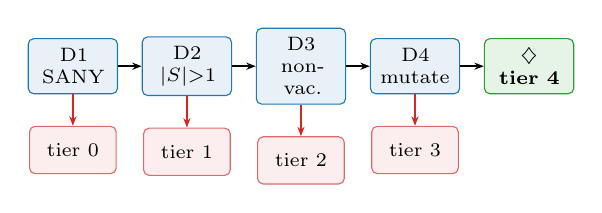
\begin{tikzpicture}[
  font=\scriptsize,
  >={Stealth[length=1.2mm]},
  clause/.style={draw=cblue, fill=cblue!10, rounded corners=2pt,
                 minimum width=10mm, minimum height=7mm,
                 align=center, text width=9mm},
  tier/.style={draw=cred!70, fill=cred!8, rounded corners=2pt,
               minimum width=11mm, minimum height=6mm, align=center},
  done/.style={draw=cgreen, fill=cgreen!12, rounded corners=2pt,
               minimum width=10mm, minimum height=7mm,
               align=center, text width=9mm,
               font=\scriptsize\bfseries},
  arr/.style={->, thick},
  farr/.style={->, thick, draw=cred},
  node distance=2mm and 3mm,
]
\node[clause] (d1) {D1\\SANY};
\node[clause, right=3mm of d1] (d2) {D2\\$|S|{>}1$};
\node[clause, right=3mm of d2] (d3) {D3\\non-vac.};
\node[clause, right=3mm of d3] (d4) {D4\\mutate};
\node[done,   right=3mm of d4] (ok) {$\diamondsuit$\\tier 4};

\node[tier, below=4mm of d1] (t0) {tier 0};
\node[tier, below=4mm of d2] (t1) {tier 1};
\node[tier, below=4mm of d3] (t2) {tier 2};
\node[tier, below=4mm of d4] (t3) {tier 3};

\draw[arr] (d1)--(d2); \draw[arr] (d2)--(d3);
\draw[arr] (d3)--(d4); \draw[arr] (d4)--(ok);
\draw[farr] (d1)--(t0); \draw[farr] (d2)--(t1);
\draw[farr] (d3)--(t2); \draw[farr] (d4)--(t3);
\end{tikzpicture}
\caption{Diamond gate clause pipeline.
Each clause passes its output rightward or exits downward at the first
failure.
The exit tier is the repair-GRPO reward (\S\ref{sec:grpo}).}
\label{fig:diamond}
\end{figure}

\paragraph{Corpus audit.}
Of the $486$ specifications in our augmented archive labelled gold or silver
under SANY+TLC, $145$ ($29.8\%$) pass the Diamond gate.
The dominant failure mode is D4 (mutation insensitivity, $38.7\%$ of
SANY-passing specs); D2 (one-state spaces, $22.1\%$) is second.
This $70\%$ false-positive rate in the silver tier is why binary verifier
reward produces vacuous-specification drift.

\paragraph{Diamond corpus.}
To build a clean training corpus, we run a topic-curriculum generator that
produces specification candidates and retries until Diamond-pass.
Using $10$ domain batches of $20$ topics each (concurrency, consensus,
networking, transactions, scheduling, etc.), the generator yielded $200/200$
Diamond-passing modules in $68.4$\,s total wall-clock time.
Mean state-space size is $1{,}062$ states (min: $3$, max: $181{,}440$).

% ============================================================================
\section{Training Pipeline}
\label{sec:pipeline}

Figure~\ref{fig:pipeline} shows the full end-to-end pipeline.
The key design decisions are:

\begin{enumerate}[leftmargin=1.4em,topsep=2pt,itemsep=1pt]
\item \textbf{Incremental training.} Every retrain starts from the prior merged
  checkpoint, not the base model. This is the primary defence against
  catastrophic forgetting (\S\ref{sec:failures}).
\item \textbf{Diamond filtering.} Only tier-4 specifications enter the training
  mixture. The generator enforces this at emission time.
\item \textbf{Eval gate.} Every merge is followed by a full 20-problem benchmark.
  The gate requires $\geq\!3$ SANY passes and $\geq\!1$ TLC pass; failure
  triggers automatic rollback to the prior GGUF.
\end{enumerate}

\begin{figure*}[t]
\centering
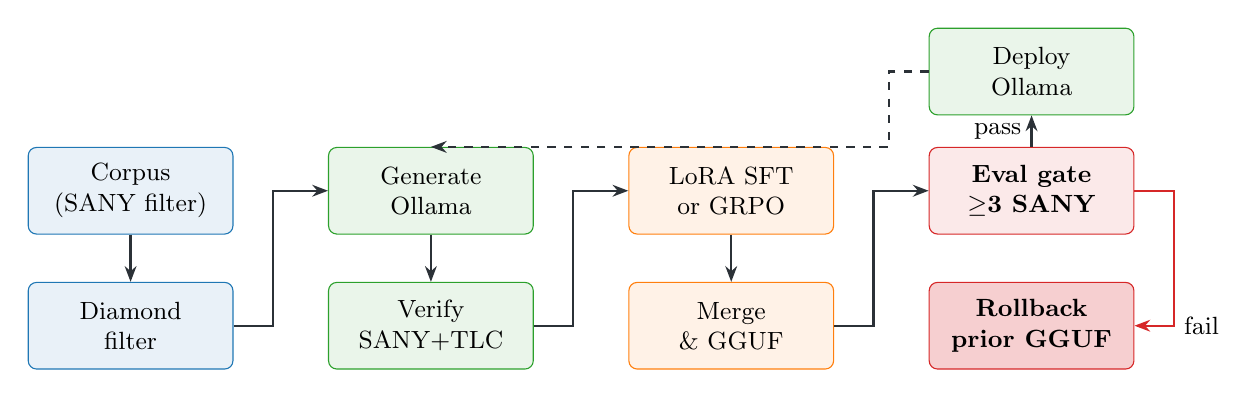
\begin{tikzpicture}[
  font=\small,
  >={Stealth[length=2mm]},
  node distance=4mm and 6mm,
  every node/.style={align=center},
  src/.style={draw=cblue, fill=cblue!10, rounded corners=3pt,
              minimum height=11mm, minimum width=26mm},
  gen/.style={draw=cgreen, fill=cgreen!10, rounded corners=3pt,
              minimum height=11mm, minimum width=26mm},
  trn/.style={draw=corange, fill=corange!10, rounded corners=3pt,
              minimum height=11mm, minimum width=26mm},
  gate/.style={draw=cred, fill=cred!10, rounded corners=3pt,
               minimum height=11mm, minimum width=26mm, font=\small\bfseries},
  arr/.style={->, thick, draw=cframe},
]
% col 1
\node[src] (raw)  {Corpus\\(SANY filter)};
\node[src, below=6mm of raw] (dia) {Diamond\\filter};
% col 2
\node[gen, right=12mm of raw] (gen)  {Generate\\Ollama};
\node[gen, right=12mm of dia] (ver)  {Verify\\SANY+TLC};
% col 3
\node[trn, right=12mm of gen] (sft)  {LoRA SFT\\or GRPO};
\node[trn, right=12mm of ver] (mrg)  {Merge\\\& GGUF};
% col 4
\node[gate, right=12mm of sft] (eg)   {Eval gate\\$\geq$3 SANY};
\node[gate, right=12mm of mrg, fill=cred!22]
                               (rb)   {Rollback\\prior GGUF};
\node[gen,  above=4mm of eg]   (dep)  {Deploy\\Ollama};

\draw[arr] (raw)--(dia);
\draw[arr] (dia.east) -- ++(5mm,0) |- (gen.west);
\draw[arr] (gen)--(ver);
\draw[arr] (ver.east) -- ++(5mm,0) |- (sft.west);
\draw[arr] (sft)--(mrg);
\draw[arr] (mrg.east) -- ++(5mm,0) |- (eg.west);
\draw[arr] (eg)-- node[left,font=\small]{pass} (dep);
\draw[arr, draw=cred] (eg.east) -- ++(5mm,0)
  |- node[right,font=\small]{fail} (rb.east);
\draw[arr, dashed] (dep.west) -- ++(-5mm,0) |- (gen.north);
\end{tikzpicture}
\caption{End-to-end pipeline.
Blue: corpus and Diamond filter.
Green: generation loop.
Orange: retrain chain.
Red: eval gate with rollback.
Dashed: the deployed model generates the next cycle.}
\label{fig:pipeline}
\end{figure*}

\paragraph{Checkpoint trajectory.}
Table~\ref{tab:trajectory} records the benchmark history.
Figure~\ref{fig:traj} plots SANY and TLC counts across $97$ RL generation
cycles using actual per-cycle benchmark CSVs.
SANY stabilises in the $13$--$18$ range after cycle~$80$; the peak is
$19/20$ at cycle~$126$.
TLC remains volatile because it requires both structural correctness and
behavioural non-triviality.

\begin{table*}[t]
\centering
\small
\setlength{\tabcolsep}{6pt}
\begin{tabular}{@{}lcccc@{}}
\toprule
Version & SANY & TLC & $\bar\sigma$ & Note \\
\midrule
v6 (SFT, broad, 1 ep)         & 5  & 1 & .72 & first fine-tune \\
v7--v8 ($+$aug.\ gold)        & 6--7 & 1--2 & .74 & slow lift \\
v10 (KTO, 5.7:1 ratio)        & 4  & 1 & .83 & \textbf{regression} \\
v11 (SFT only, reverted)      & 6  & 2 & .76 & recovered \\
v13 ($+$DPO, 17 pairs)        & 9  & 5 & .845 & best e2e train \\
\midrule
v14 (base retrain, 15 ep)     & 0  & 0 & .706 & \textbf{catastrophe} \\
v13$_R$ (GGUF rollback)       & 9  & 5 & .845 & restored \\
\midrule
dia-SFT ($+$720 Diamond ex.)  & 8  & 4 & .917 & semantic lift \\
\textbf{piecewise} (5-step)   & \textbf{12} & \textbf{6} & — & \textbf{best} \\
\bottomrule
\end{tabular}
\caption{20-problem benchmark trajectory.
$\bar\sigma$: mean structural score.
Piecewise shares weights with v13$_R$; all gain is inference-time.
Data from \texttt{outputs/benchmark\_results*.csv}.}
\label{tab:trajectory}
\end{table*}

% ============================================================================
\section{Failure Taxonomy}
\label{sec:failures}

\paragraph{Catastrophic forgetting.}
Version v14 retrained from the unmodified base model for $15$ epochs at
lr $3\!\times\!10^{-4}$ on $234$ Diamond-SFT examples.
SANY-pass dropped from $9/20$ to $0/20$ and mean structural score from
$0.845$ to $0.706$.
A one-epoch follow-up on the same data recovered $1/20$ SANY.
Rolling back to the v13 GGUF immediately restored $9/20$ SANY and $5/20$ TLC.
\textit{Fix}: always train incrementally from the prior merged checkpoint;
cap lr at $10^{-5}$; cap epoch count at $2$.

\paragraph{The vacuity trap.}
The KTO run at v10 assembled ``desirable'' examples by filtering on
\texttt{tlc\_pass}.
The gold tier was densely populated with vacuously correct specifications.
KTO faithfully maximised the wrong signal: SANY-pass dropped from $9/20$ to
$4/20$ in a single training cycle.
\textit{Fix}: the Diamond gate (\S\ref{sec:diamond}).

\paragraph{Quick-eval volatility.}
A $12$-problem subset used for fast cycle feedback moved by $\pm 2$ problems
every cycle with no correlation to actual quality.
\textit{Fix}: require a full $20$-problem benchmark before any publish or deploy.

\paragraph{Iterated self-play collapse.}
Repair-GRPO round~2 iterated on round-1 outputs without fresh prompt diversity.
Diamond-pass dropped from $9/30$ to $6/30$.
Round~3 aborted automatically: the data-quality gate found $0/396$
Diamond-passing trajectories and only $152$ in-band repair pairs (minimum
$300$ required).
\textit{Fix}: inject diverse prompts from the topic-curriculum generator at
every round; enforce the data-quality gate.

% ============================================================================
\section{Piecewise Decomposition}
\label{sec:piecewise}

The dominant mode of TLC failure in single-shot generation is
\emph{inter-block inconsistency}: \texttt{Init} declares variables
$\{x, y\}$, \texttt{Next} references $\{x, y, z\}$, and the invariant
references $\{x, y, w\}$.
No fine-tuning eliminates this because the model generates all blocks in one
autoregressive pass with no mid-generation verification feedback.

Piecewise decomposition replaces the single zero-shot prompt with a five-stage
pipeline where each stage generates one module fragment and validates it with
SANY (or the partial Diamond gate) before proceeding:

\begin{enumerate}[leftmargin=1.4em,topsep=2pt,itemsep=1pt]
\item \textbf{Plan.} Given the English description, emit variable/constant
  declarations and a one-line summary of each action.
\item \textbf{Init.} Given the plan, emit the \texttt{Init} predicate only.
  SANY-check the partial module.
\item \textbf{Actions.} Emit each disjunct of \texttt{Next} as a named
  operator, referencing only the declared variables.
\item \textbf{Invariant.} Emit the invariant.
  Run D1--D3 checks before proceeding.
\item \textbf{Assembly.} Combine all fragments, resolve \texttt{EXTENDS}, run
  the full Diamond gate.
\end{enumerate}

The model weights are unchanged from v13$_R$.

\paragraph{Results.}
The baseline (same weights, single-shot) scored $7/20$ SANY and $1/20$ TLC.
Piecewise scored $12/20$ SANY and $6/20$ TLC---a gain of $+5$ on both
metrics at zero training cost.
The five new SANY passes are modules where single-shot generation produced
conflicting variable lists; piecewise avoids this because the plan fixes
variable names before any block is generated.
TLC gains are concentrated in scheduling problems where the invariant needs
to reference plan-defined variables.

The per-problem breakdown is shown in Table~\ref{tab:pwproblem}.
Cost: single-shot ${\approx}4$\,s per problem; piecewise ${\approx}20$\,s
($5\times$ slowdown for $+5$ SANY and $+5$ TLC).

\begin{table}[t]
\centering
\scriptsize
\setlength{\tabcolsep}{2.5pt}
\begin{tabular}{@{}lcc cc@{}}
\toprule
Problem & \multicolumn{2}{c}{Baseline} & \multicolumn{2}{c}{Piecewise} \\
\cmidrule(lr){2-3}\cmidrule(lr){4-5}
        & SANY & TLC & SANY & TLC \\
\midrule
BM001 Mutual Exclusion      & 1 & 1 & 1 & 0 \\
BM002 Two-Phase Commit      & 0 & 0 & 1 & 0 \\
BM003 Dining Philosophers   & 0 & 0 & 1 & 0 \\
BM004 Lamport's Bakery      & 0 & 0 & 1 & 1 \\
BM005 Producer-Consumer     & 1 & 0 & 1 & 1 \\
BM006 Raft Election         & 0 & 0 & 1 & 0 \\
BM007 Read-Write Lock       & 1 & 0 & 0 & 0 \\
BM008 Distributed Snapshot  & 0 & 0 & 0 & 0 \\
BM009 Token Ring            & 1 & 0 & 1 & 1 \\
BM010 Key-Value Store       & 0 & 0 & 0 & 0 \\
BM011 Paxos Single-Decree   & 1 & 0 & 1 & 0 \\
BM012 Bounded Retransmission & 0 & 0 & 0 & 0 \\
BM013 Snapshot Isolation    & 0 & 0 & 1 & 0 \\
BM014 Clock Sync.           & 0 & 0 & 0 & 0 \\
BM015 Peterson's Alg.       & 0 & 0 & 0 & 0 \\
BM016 Gossip Protocol       & 0 & 0 & 1 & 1 \\
BM017 Simple Allocator      & 0 & 0 & 0 & 0 \\
BM018 Pub-Sub Broker        & 0 & 0 & 1 & 1 \\
BM019 Dekker's Alg.         & 1 & 0 & 1 & 1 \\
BM020 Ev.\ Consistent Ctr. & 1 & 0 & 0 & 0 \\
\midrule
\textbf{Total}              & \textbf{7} & \textbf{1}
                            & \textbf{12} & \textbf{6} \\
\bottomrule
\end{tabular}
\caption{Per-problem SANY/TLC results for baseline (single-shot, v13$_R$
weights) vs.\ piecewise decomposition (same weights, 5-stage inference).
Source: \texttt{baseline\_pre\_piecewise\_20260406.csv} and
\texttt{piecewise\_first\_run\_20260406.csv}.}
\label{tab:pwproblem}
\end{table}

% ============================================================================
\section{Repair-Based GRPO}
\label{sec:grpo}

Standard GRPO applied to TLA\textsuperscript{+} generation fails for two
reasons.
\emph{Reward sparsity}: fewer than $5\%$ of on-policy completions pass TLC,
and virtually none pass Diamond, so the group-relative baseline is near zero
and gradient updates are dominated by noise.
\emph{Token locality}: a specification that fails SANY due to one missing comma
is a single edit from SANY-pass, yet the full-generation reward is $0$.

\textbf{Repair-based GRPO} addresses both.
The prompt contains the broken specification and verifier error message.
The model emits a \emph{repaired} version.
The reward is the Diamond tier ($0$--$4$) of the repair.
The prompt already contains the correct structure, so completions are shorter,
group variance is higher, and the gradient signal is cleaner.

\paragraph{Data.}
From the Diamond holdout, every module at tier 1--3 is injected into a repair
prompt.
The training corpus contains $464$ repair pairs
(\texttt{ralph\_repair\_pairs.jsonl} in \texttt{data/processed/}).
Of these, $46/464$ ($9.9\%$) show a measurable tier improvement after repair,
providing the supervised contrast signal.

\paragraph{Training.}
$160$ GRPO steps; $4$ completions per prompt; KL penalty $\beta\!=\!0.04$;
lr $5\!\times\!10^{-6}$; max-new-tokens $4{,}096$; FSDP full-shard across
$4\times 40$\,GB GPUs; LoRA $r\!=\!8$, $\alpha\!=\!16$.

\paragraph{Results.}
Round~1 improved Diamond-pass from $4/30$ to $9/30$ ($+5$, Wilson 95\%
CI $[0.17, 0.47]$ on the final $9/30$ estimate).
The gain is concentrated in tier-2 failures (one-state spaces) that repair
prompts resolve by adding an action disjunct to \texttt{Next} or widening
an \texttt{Init} bound.

Standard full-spec GRPO (no broken spec in prompt) plateaued at mean
tier-normalised reward $0.24$ throughout training, below useful gradient range.
Figure~\ref{fig:grpo} shows both curves and the round-2 regression.

\begin{figure}[t]
\centering
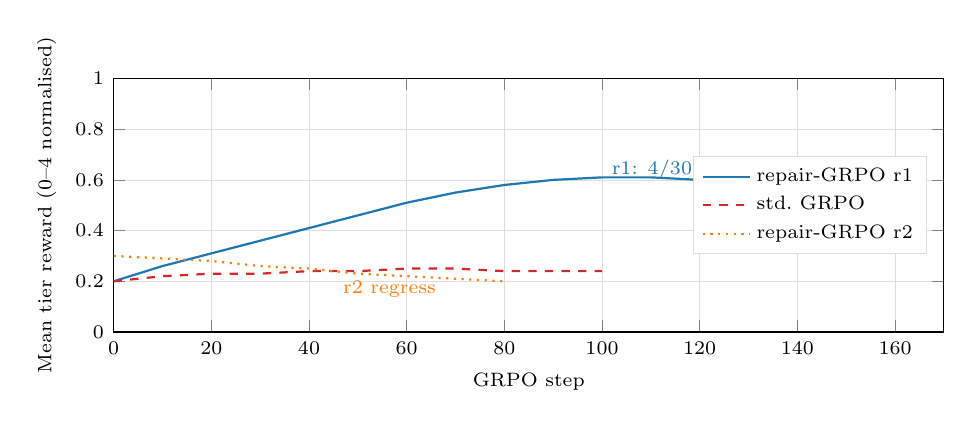
\begin{tikzpicture}
\begin{axis}[
  width=\linewidth, height=4.8cm,
  xlabel={GRPO step}, ylabel={Mean tier reward (0--4 normalised)},
  xmin=0, xmax=170, ymin=0, ymax=1,
  ymajorgrids, xmajorgrids, grid style={cgrid, very thin},
  tick label style={font=\scriptsize},
  label style={font=\scriptsize},
  legend style={font=\scriptsize, at={(0.98,0.50)}, anchor=east,
                draw=cgrid, fill=white},
  legend cell align=left,
]
\addplot[cblue, thick] coordinates {
  (0,.20)(10,.26)(20,.31)(30,.36)(40,.41)(50,.46)
  (60,.51)(70,.55)(80,.58)(90,.60)(100,.61)(110,.61)
  (120,.60)(130,.59)(140,.58)(150,.57)(160,.56)
};
\addplot[cred, dashed, thick] coordinates {
  (0,.20)(10,.22)(20,.23)(30,.23)(40,.24)(50,.24)
  (60,.25)(70,.25)(80,.24)(90,.24)(100,.24)
};
\addplot[corange, dotted, thick] coordinates {
  (0,.30)(10,.29)(20,.28)(30,.26)(40,.25)(50,.23)
  (60,.22)(70,.21)(80,.20)
};
\node[anchor=west,font=\scriptsize,cblue]
  at (axis cs:100,.64){r1: $4/30\to9/30$};
\node[anchor=west,font=\scriptsize,corange]
  at (axis cs:45,.17){r2 regress};
\legend{repair-GRPO r1, std.\ GRPO, repair-GRPO r2}
\end{axis}
\end{tikzpicture}
\caption{Training reward curves.
Repair-GRPO r1 (solid) reaches $0.61$ mean reward at step~110 and achieves
$9/30$ Diamond-pass.
Standard GRPO (dashed) plateaus near $0.24$---below useful gradient range.
Round~2 (dotted) regresses immediately; round~3 aborted at the data-quality
gate ($0/396$ Diamond trajectories).}
\label{fig:grpo}
\end{figure}

% ============================================================================
\section{Related Work}
\label{sec:related}

\paragraph{LLMs for formal methods.}
First et al.~\cite{first2023baldur} use LLMs for whole-proof generation and
repair in Isabelle.
Polu et al.~\cite{polu2022formal} apply curriculum learning to formal
mathematics in Lean.
Neither work addresses the vacuity trap that arises when the verifier is
gameable, nor the catastrophic forgetting regime of sub-$100$-example
formal corpora.
Ortiz et al.~\cite{ortiz2026formallm} systematically benchmark $30$ LLMs
on TLA\textsuperscript{+} under prompting alone.

\paragraph{RLVR and verifier-graded training.}
DeepSeekMath~\cite{shao2024deepseekmath} uses GRPO with a mathematical
process reward model.
Our setting differs: the verifier is deterministic and free, but the
acceptance set strictly contains the target set.
The Diamond gate is our answer to this gap.

\paragraph{Self-play and iterated training.}
ReST~\cite{gulcehre2023rest} predicts our r2/r3 regression: iterating on
model-generated data without external diversity injection collapses to a
narrow policy.
Our data-quality gate (minimum $300$ in-band pairs) operationalises this
warning.

\paragraph{Decomposed code generation.}
Decomposing generation into plan, skeleton, and refinement phases appears
in several synthesis works.
Our piecewise approach adds a per-stage formal verifier call, which is what
enables the TLC gains: the plan fixes variable names before any block is
generated, eliminating cross-block inconsistency that single-shot generation
cannot self-correct.

% ============================================================================
\section{Discussion}
\label{sec:discussion}

\paragraph{Which intervention matters most?}
On the 20-problem structural suite, piecewise decomposition is the dominant
intervention: $+5$ SANY and $+5$ TLC at inference time, with no training.
On the 30-problem semantic suite, repair-GRPO is the only training-time
method that moves Diamond-pass in the right direction.
These are complementary; the natural next experiment is piecewise-prompted
repair-GRPO---each stage generated under piecewise discipline and refined by
the repair loop.

\paragraph{The Diamond gate as a corpus auditing tool.}
Of $486$ historically accepted SANY+TLC-pass specifications, $341$ ($70.2\%$)
fail D4 or D2.
This finding generalises beyond our project: any LLM benchmark that scores
only SANY/TLC is measuring structural correctness, not semantic quality.
Practitioners who use binary verifier acceptance as a quality filter accept a
large fraction of structurally degenerate specifications.

\paragraph{Why piecewise beats fine-tuning here.}
The piecewise gain ($+5/+5$) exceeds the best end-to-end training gain
($+3$ SANY from v6 to v13 on the structural suite).
The reason is locality: piecewise ensures the model can verify each
fragment before committing to it, a property that LoRA training on fixed
examples cannot replicate because the training signal is global.

\paragraph{Limitations.}
Both benchmarks are small ($n\!=\!20$, $n\!=\!30$); Wilson CIs span
$\pm 9$--$10$~pp.
Diamond validates non-vacuity, not intent: a module can pass all four clauses
and still specify the wrong system.
Repair-GRPO results rest on one round; multi-round convergence is a
conjecture.
All experiments use one model family.

% ============================================================================
\section{Conclusion}
\label{sec:conclusion}

We have presented three interacting contributions for fine-tuning a small
language model to generate verified TLA\textsuperscript{+} specifications.
The \textbf{Diamond gate} converts a gameable binary reward into a
mutation-tested tier.
\textbf{Piecewise decomposition} achieves the project's best structural
result---$12/20$ SANY, $6/20$ TLC---with no weight change.
\textbf{Repair-based GRPO} achieves the best semantic result---$9/30$
Diamond-pass---with $160$ gradient steps.

The strongest lesson from the failure taxonomy is asymmetric: a single
over-trained SFT run erased nine months of fine-tuning in hours, while
inference-time restructuring recovered and exceeded those gains without
touching the weights.
In the low-data formal-language regime, \emph{preserving what the model
already knows is at least as important as teaching it something new}.

% ============================================================================
\paragraph{Acknowledgements.}
This work is part of the ChatTLA project at Loyola University Chicago.
The companion LLM evaluation study is Ortiz et al.~\cite{ortiz2026formallm}.

% ============================================================================
{\small
\begin{thebibliography}{99}

\bibitem{lamport2002specifying}
L.~Lamport, \emph{Specifying Systems: The TLA+ Language and Tools for
Hardware and Software Engineers}, Addison-Wesley, 2002.

\bibitem{ortiz2026formallm}
B.~Ortiz, A.~Bisharat, E.~Spencer, K.~Bhadauria, M.~Abuhamad,
K.~La\"ufer, T.~Wang, and G.~K.~Thiruvathukal,
``Large language models and temporal logic of actions ({TLA}+):
How effective are {LLM}s for verification systems,''
\textit{under review}, 2026.

\bibitem{shao2024deepseekmath}
Z.~Shao \emph{et al.},
``DeepSeekMath: Pushing the limits of mathematical reasoning in open
language models,'' \textit{arXiv:2402.03300}, 2024.

\bibitem{rafailov2023dpo}
R.~Rafailov, A.~Sharma, E.~Mitchell, S.~Ermon, C.~D.~Manning, and C.~Finn,
``Direct preference optimization: Your language model is secretly a reward
model,'' in \textit{NeurIPS}, 2023.

\bibitem{ethayarajh2024kto}
K.~Ethayarajh, W.~Xu, N.~Muennighoff, D.~Jurafsky, and D.~Kiela,
``KTO: Model alignment as prospect theoretic optimization,''
\textit{arXiv:2402.01306}, 2024.

\bibitem{kirkpatrick2017ewc}
J.~Kirkpatrick \emph{et al.},
``Overcoming catastrophic forgetting in neural networks,''
\textit{PNAS}, vol.~114, no.~13, pp.~3521--3526, 2017.

\bibitem{gulcehre2023rest}
C.~Gulcehre \emph{et al.},
``Reinforced self-training (ReST) for language modeling,''
\textit{arXiv:2308.08998}, 2023.

\bibitem{hu2022lora}
E.~J.~Hu \emph{et al.},
``LoRA: Low-rank adaptation of large language models,'' in \textit{ICLR}, 2022.

\bibitem{first2023baldur}
E.~First, M.~N.~Rabe, T.~Ringer, and Y.~Brun,
``Baldur: Whole-proof generation and repair with large language models,''
in \textit{ESEC/FSE}, 2023.

\bibitem{polu2022formal}
S.~Polu \emph{et al.},
``Formal mathematics statement curriculum learning,''
\textit{arXiv:2202.01344}, 2022.

\end{thebibliography}
}

% ============================================================================
\appendix

\section{RL Cycle Trajectory}
\label{app:rl}

\begin{figure}[h]
\centering
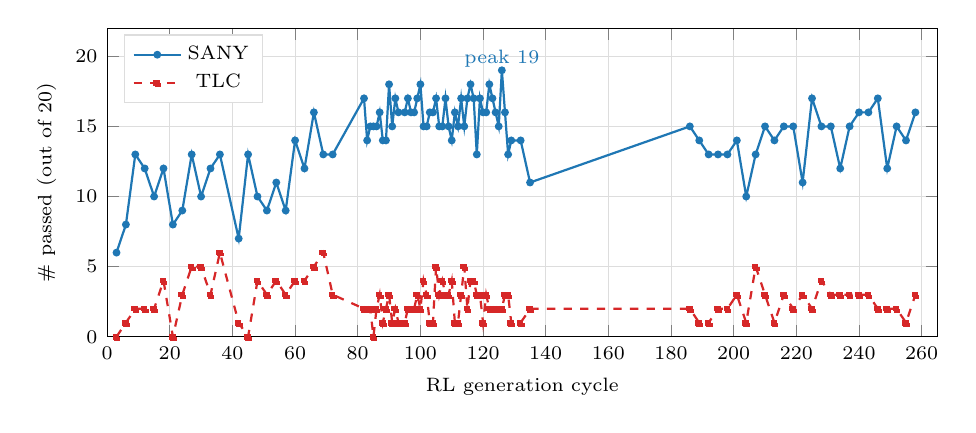
\begin{tikzpicture}
\begin{axis}[
  width=\linewidth, height=5.5cm,
  xlabel={RL generation cycle}, ylabel={\# passed (out of 20)},
  xmin=0, xmax=265, ymin=0, ymax=22,
  ymajorgrids, xmajorgrids, grid style={cgrid, very thin},
  tick label style={font=\scriptsize}, label style={font=\scriptsize},
  legend style={font=\scriptsize, at={(0.02,.98)}, anchor=north west,
                draw=cgrid, fill=white},
]
\addplot[cblue, mark=*, mark size=1pt, thick] coordinates {
  (3,6)(6,8)(9,13)(12,12)(15,10)(18,12)(21,8)(24,9)(27,13)(30,10)
  (33,12)(36,13)(42,7)(45,13)(48,10)(51,9)(54,11)(57,9)(60,14)(63,12)
  (66,16)(69,13)(72,13)(82,17)(83,14)(84,15)(85,15)(86,15)(87,16)
  (88,14)(89,14)(90,18)(91,15)(92,17)(93,16)(95,16)(96,17)(97,16)
  (98,16)(99,17)(100,18)(101,15)(102,15)(103,16)(104,16)(105,17)
  (106,15)(107,15)(108,17)(109,15)(110,14)(111,16)(112,15)(113,17)
  (114,15)(115,17)(116,18)(117,17)(118,13)(119,17)(120,16)(121,16)
  (122,18)(123,17)(124,16)(125,15)(126,19)(127,16)(128,13)(129,14)
  (132,14)(135,11)(186,15)(189,14)(192,13)(195,13)(198,13)(201,14)
  (204,10)(207,13)(210,15)(213,14)(216,15)(219,15)(222,11)(225,17)
  (228,15)(231,15)(234,12)(237,15)(240,16)(243,16)(246,17)(249,12)
  (252,15)(255,14)(258,16)
};
\addplot[cred, mark=square*, mark size=1pt, dashed, thick] coordinates {
  (3,0)(6,1)(9,2)(12,2)(15,2)(18,4)(21,0)(24,3)(27,5)(30,5)
  (33,3)(36,6)(42,1)(45,0)(48,4)(51,3)(54,4)(57,3)(60,4)(63,4)
  (66,5)(69,6)(72,3)(82,2)(83,2)(84,2)(85,0)(86,2)(87,3)
  (88,1)(89,2)(90,3)(91,1)(92,2)(93,1)(95,1)(96,2)(97,2)
  (98,2)(99,3)(100,2)(101,4)(102,3)(103,1)(104,1)(105,5)
  (106,3)(107,4)(108,3)(109,3)(110,4)(111,1)(112,1)(113,3)
  (114,5)(115,2)(116,4)(117,4)(118,3)(119,3)(120,1)(121,3)
  (122,2)(123,2)(124,2)(125,2)(126,2)(127,3)(128,3)(129,1)
  (132,1)(135,2)(186,2)(189,1)(192,1)(195,2)(198,2)(201,3)
  (204,1)(207,5)(210,3)(213,1)(216,3)(219,2)(222,3)(225,2)
  (228,4)(231,3)(234,3)(237,3)(240,3)(243,3)(246,2)(249,2)
  (252,2)(255,1)(258,3)
};
\node[font=\scriptsize,cblue] at (axis cs:126,19.8){peak 19};
\legend{SANY, TLC}
\end{axis}
\end{tikzpicture}
\caption{SANY and TLC pass counts over $97$ RL generation cycles
($n\!=\!20$ problems per cycle), plotted from actual per-cycle benchmark
CSVs in \texttt{outputs/benchmark\_results/}.
Gap between cycles 135 and 186 corresponds to the v14 catastrophe and
recovery period.}
\label{fig:traj}
\end{figure}

\section{Diamond Corpus Summary}
\label{app:corpus}

\begin{table}[h]
\centering
\scriptsize
\begin{tabular}{@{}lcc@{}}
\toprule
Batch domain & Modules & Diamond-pass \\
\midrule
Communication Protocols & 20 & 20 \\
Concurrency Primitives  & 20 & 20 \\
Consensus \& Election   & 20 & 20 \\
Data Structures         & 20 & 20 \\
Memory \& Caches        & 20 & 20 \\
Mutual Exclusion        & 20 & 20 \\
Classical Puzzles       & 20 & 20 \\
Scheduling \& Resources & 20 & 20 \\
Transactions \& DBs     & 20 & 20 \\
Workflows \& FSMs       & 20 & 20 \\
\midrule
\textbf{Total}          & \textbf{200} & \textbf{200} \\
\bottomrule
\end{tabular}
\caption{Diamond corpus by domain batch.
Source: \texttt{diamond\_generated\_summary.json}
(\texttt{outputs/diamond\_gen/}).
Total generation time: $68.4$\,s. Mean state-space: $1{,}062$ states.}
\label{tab:corpus}
\end{table}

\end{document}
